\documentclass[fleqn,10pt]{SelfArx}
\setlength{\columnsep}{0.55cm}
\setlength{\fboxrule}{0.75pt}  
\definecolor{color1}{RGB}{0,0,90}
\definecolor{color2}{RGB}{0,20,20}
\newlength{\tocsep} 
\setlength\tocsep{1.5pc}
\setcounter{tocdepth}{3}
%\usepackage{lipsum}

%----------------------------------------------------------------------------------------
%	ARTICLE INFORMATION
%----------------------------------------------------------------------------------------

\JournalInfo{Students Journal of AI, IIT, Jodhpur, Vol. 1, No. 1, 2014} 
\Archive{Tracking solutions of sudoku puzzles}

\PaperTitle{AI for Solving Sudoku Puzzles} % Article title

\Authors{Praneeth A S, UG201110023\textsuperscript{1}} % Authors
\affiliation{\textsuperscript{1}\textit{Department of Computer Science \& Engineering, Indian Institute of Technology, Jodhpur, India}} 

\Keywords{AI, Sudoku Solving, Games}
\newcommand{\keywordname}{Keywords}
%----------------------------------------------------------------------------------------
%	ABSTRACT
%----------------------------------------------------------------------------------------

\Abstract{Sudoku is a game popular in Japan. It requires filling of an $n \times n$ square grid with $1$ to $n$ values such that every row, column has numbers from $1$ to $n$. THe entire square is divided into n sub-regions of dimension = $\sqrt{n}$. This paper aims at providing various methods of solvinfg sudoku puzzles using artificial intelligence techniques.}

%----------------------------------------------------------------------------------------

\begin{document}

\flushbottom % Makes all text pages the same height

\maketitle % Print the title and abstract box

\tableofcontents % Print the contents section

\thispagestyle{empty} % Removes page numbering from the first page

%----------------------------------------------------------------------------------------
%	ARTICLE CONTENTS
%----------------------------------------------------------------------------------------

\section{Introduction}  

\addcontentsline{toc}{section}{\hspace*{-\tocsep}Introduction}  

\textbf{Sudoku} is a popular number game in \textbf{Japan}. This game involves a $9 \times 9$ square grid in which the values from $1$ to $9$ are filled into the squares. The puzzle setter provides a partially completed grid, which typically has a unique solution. The sqaures should be filled such that every row has a number from $1$ to $9$, every column has a number from $1$ to $9$. Additionally, this square is divided into $9$ sub-regions of dimension $3 \times 3$. Even these sub-regions should have numbers from $1$ to $9$.
%------------------------------------------------

\begin{figure*}[ht]\centering 
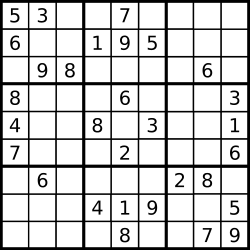
\includegraphics[scale=0.6]{sudoku.png}
\caption{Standard $9 \times 9$ Sudoku grid}
\label{fig:view}
\end{figure*}


\section{Objective}

This paper evaluates various techniques for solving Sudoku puzzles by a machine. We would be learning sudoku puzzles of various dimensions which would be solved using artificial intelligence techniques like backtracking, genetic algorithms, simulated annealing etc.,

\section{Motivation}

This project is a challenging project. Though solving sudoku puzzles would be easier for smaller dimensions but becomes increasingly difficult for more larger dimensions of $n$. Ordinary methods of brute force would become completely inefficient for solving. So it is essential to optimize methods for solving this problem in order to save on time and space.

\section{Theory}
Sudoku is a kind of constraint satisfaction problem (CSP); a problem whose solution requires a set of variables and which imposes constraints on the values they can take.

\section{Algorithms}
\subsection{Guessing at random}
This procedure is a naive one where we guess a number between $1$ \& $n$ and place it in the square we wish to. If it doesnot violate any constraints then we place it in the square, else we don't.
This method is a worst one as it would take alot of time for solving a veru huge grid. It is even guaranteed to find a valid solution - given enough time - because it will eventually try all
of them. The catch of course is the time required. In the worst case it requires infinite time to find
a correct solution, because only then is it guaranteed that every possible solution will be generated.
\subsection{Exhaustive Search}
The next simplest way to search for a valid solution to a puzzle is to enumerate (that is, generate
all possible instances of) the unconstrained grids. After generating each new grid you check to see
whether it’s a valid solution, and if so you’re done. This algorithm is guaranteed to find a solution
since it will check all grids if need be, but in the worst case the only solution is the last grid it checks.
We call this an exhaustive search since it exhausts all the possibilities (and anyone who tries to do it
by hand).

\begin{figure*}[ht]\centering 
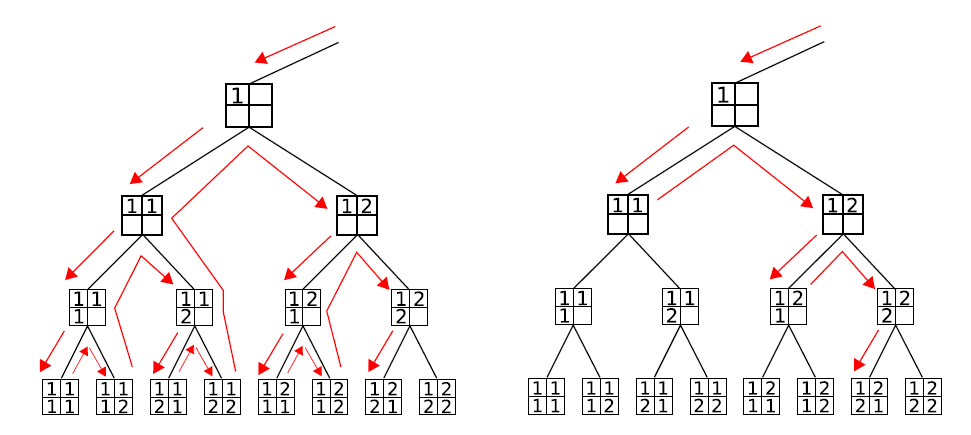
\includegraphics[scale=0.5]{BackTrack.PNG}
\caption{Backtrack search for $2 \times 2$ Sudoku grid}
\label{fig:view}
\end{figure*}


\subsection{Backtracking Search}
Pick the first empty square
and assign $1$ to that square. If the one conflicts with another value, then change it to a two. Keep
doing this until a value that does not conflict is found. Once a value that does not conflict has been
found, pick another square and repeat this process. If a square has no possible values, then return to
the previously assigned square and change its value. This method of search is known as a
backtracking search.It is guaranteed to find a solution if there is one,simply because it will eventually try every possible number in every possible location. This
algorithm is very effective for size two puzzles. Unfortunately for size three puzzles there are nine
possibilities for each square. This means that there are roughly $9^{81-n}$ possible states that might
need to be searched, where n is number of given values. Obviously this version of backtracking
search is not going to work for size 3 puzzles. Fortunately there are several means by which this
algorithm can be improved: constraint propagation, forward checking and choosing most
constrained value first.
\subsubsection{Forward Checking}
The first improvement on backtracking search is forward checking. Notice that the old
version of backtracking search had to place a value and then check for conflicts. Instead it is easier
to just maintain a list of which possible values each square can possibly have given the other
numbers that have been assigned. Then when the values are being assigned to that square, only
consider the ones that do not directly conflict with the other already placed numbers. For a size
three puzzle forward checks can be stored in a nine by nine by nine boolean array. Basically each
square has its own array of nine boolean values corresponding to each of the numbers that could
possibly go in that square. If the third value in the array is set to false, then that square cannot
contain a three. Maintaining these lists is simple. Whenever a new value x is assigned is assigned,
go to every other square in the same row, column and box and mark false in its array for value x.
Storing this information can be used in two ways. First, it can be used to verify that no value is ever
assigned that directly conflicts with another assigned value. Second, if the array for any square
contains all false values, then there is no possible value for that square and the most recently
assigned value is wrong. Using forward checking the backtracking search can now solve size three
puzzles.
\subsubsection{Minimum Remaining Values}
Another method for improving the backtracking search is the minimum remaining values
heuristic. The minimum remaining values heuristic is used to alter the
order in which squares are guessed in order to reduce the number of branches at each level.
Basically instead of choosing the first empty square, the square with the least number of possible
values is chosen. By choosing the square with only two possible values instead of three the search tree only
branches in two directions instead of three. Basically the search tree is reduced in size by a factor of
two thirds.
\subsubsection{Hill Climbing}
Given the size of the state space it is logical to use a search method with a heuristic function
to avoid searching less promising sections of the state space. One type algorithm that meets thiscriteria is hill climbing. Hill climbing algorithms work by generating a list of successors of the
current state, then choosing the one with the lowest heuristic value. In order to apply hill climbing
to Sudoku three things must be defined: the start state, the successor function and the heuristic
function. One way to go about this is to fill in each box so that it contains the numbers one to $n^2$ and
allow successors to be generated by switching values within the same box. Instead of
filling in the boxes with the numbers one to n2 the rows will be filled, but the idea is the same. Let
the start state be defined as the initially puzzle with all of the empty spaces filled in such that each
row contains the numbers one to n2. Using this as a start state, the successor function can be
defined as swapping any two nonfixed
values in the same row. The heuristic can simply be the sum
of the number of conflicts that appear within each column and each box. Since each row has exactly
the numbers one to n2 there are no conflicts within the rows. Hill climbing can successfully solve
size two puzzles occasionally.
\subsubsection{Random Restart}
The general hill climbing algorithm described above is incomplete. This is because it can
get stuck in a local minimum. One simple way to fix this is to randomly restart the algorithm
whenever it goes a while without improving the heuristic value. This is known as random restart
hill climbing. This version of hill climbing does not quite suffice to solve
the puzzle. The problem comes from the completely random way in which the variables are filled
in. One technique for dealing with this is to switch certain values after the initial random
placement. Known as postswapping
this technique attempts to minimize the number of values that
conflict with the values given in the original puzzle. Another possible solution is
to use the constraint propagation algorithm. Applying constraint propagation before filling in any
random values prevents some values from being randomly guessed incorrectly. Also, constraint
propagation can be applied in between the assignments of each row to make sure that the future
rows agree better with the rows that have already been assigned. This method allows most puzzles
of size three to be solved.
\subsection{Genetic Algorithm}
A genetic algorithm is a search technique used in order in computing to find exact or approximate solutions to optimization and search problems. Genetic algorithms are categorized as global search heuristics. Genetic algorithms are a particular class of evolutionary algorithms that use techniques inspired by evolutionary biology such as inheritance, mutation, selection and crossover.
\subsubsection{Some Definitions}
\begin{enumerate}
\item \underline{Gene} - an empty cell in the original Sudoku puzzle, filled with some legal value .
\item \underline{Individual/Chromosome} - an object representing a potential solution of the Sudoku problem. An individual actually consists of a sequence of genes, each of which has a value within it.
\item \underline{Population} - a set of individuals.
\item \underline{Fitness function} - a function from the space of individuals to R which represents the number of contradictions.
\end{enumerate}
\subsubsection{Implementation}
In our implementation, each individual represents a solution of the Sudoku puzzle, where each gene represents a cell which isn't fixed.
First we've created a random population of Sudoku solutions– where each individual consists only with randomly selected legal values - the value is within legal range and has no contradiction with fixed cells.
Once created, the fitness value of each member of the population is computed and the population is sorted in ascending order of fitness - when zero is the best value and represents a solution to the problem.
While there is no individual of value zero (and therefore the problem isn't solved yet), we perform selection of half of the best-valued individuals in our population, in order for them to create the next generation of solutions.
We choose randomly which two individuals mate, and create a new generation using crossover and mutation.
Given two parents we choose one random point of crossover and create two children which are a combination of their parents' genes according to crossover point.
A mutation is also performed randomly, on a recently created individual, on a random gene, by transforming the gene's value into a different but legal value.
The act of mutation helps the algorithm in avoiding local minimum solutions. However it isn't perfect, and as a result the algorithm should be restrained with a maximal number of generations created.
This cycle of life is being performed until a solution is found or until the algorithm has reached its limit regarding to number of generations created.
\subsection{Simulated Annealing}
Simulated annealing (SA) is a generic probabilistic metaheuristic for the global optimization problem of applied mathematics, namely locating a good approximation to the global minimum of a given function in a large search space… each step of the SA algorithm replaces the current solution by a random nearby solution, chosen with a probability... The allowance for uphill moves saves the method from becoming stuck at local minima.
\subsubsection{Some Definitions}
\begin{enumerate}
\item \underline{Approximated solution} - a Sudoku board, where its non-fixed cells are filled with randomly selected legal values.
\item \underline{A neighbor solution} - a solution $S^{'}$ which is close to the given solution S, differs from it only by one parameter ( in our implementation - only by a fitness value of one cell)
\item \underline{An improving value} -  a legal value which is given to a cell and improves its fitness value.
\item \underline{A downhill move} - moving to an approximated solution which has a lower fitness value than the currant solution. (In our implementation - a value of a cell is changed to a different legal value, but with a worse fitness value).
\end{enumerate}
\subsubsection{Implementation}
Given a Sudoku board we create an approximated solution – S.
Once created, the fitness value of S is being calculated alongside with the fitness value of each of the cells.
While the solution's fitness isn't zero we search for the next best step, an approximated solution which has a better fitness value.
In order to achieve this goal, we try to find an improving value to the worst cell (the one with the worst fitness value) in the board, this by testing all possible legal values.
If no legal value improves the cell's fitness, it is marked as tested, and we continue to next worst-valued cell. In case we haven't been able to find an improving value for any of the non fixed cells the algorithms outputs failure.
In case that several improving values are found – the value which improves the board's fitness the most is selected.
Once an improving value has been reached, a neighbor solution S' is created – in which the improving value is placed instead of the prior value in that cell.
At this stage our algorithm selects whether to move to the neighbor state or allow a downhill move. This choice is being made in a probabilistic way, in order to avoid local minima and expand the search space. The probability of selecting a downhill move lowers as the search advances, due to the thought that as the search advances we are closer to solving the problem.
After performing the probabilistic choice and moving to some other approximated solution, the loop of trying to find a neighbor solution with better fitness value is being performed, until a solution is found.
This loop continues until a solution to the problem is found.




%\section{Implementation}

%How this project can be implemented in real-life, for example what %tools, languages, hardware, programming you are going to use%/propose? What may be the various tests needed to ensure its %satisfactory performance, etc.

\section{Applications}

The algorithms used in this project could be used in those places where there are certain constraints \& there is huge certain search space of values from which goal is to be found out. As the above algorithm runs good for considerable value of 
$n$ it can be used for seraching for larger search trees.

\section{Conclusion and Results}

Although the Sudoku problem is a difficult constraint satisfaction problem, it is not
completely invulnerable to search methods. Puzzles of size three or less can be solved very quickly
and consistently. The backtracking search can consistently solve size three Sudoku puzzles after
considering fewer than 200 states. Considering that there are \\$6,670,903,752,021,072,936,960$ valid
Sudoku puzzles, searching only 200 of them to find a solution is excellent. Random restart hill
climbing is also successful on easy puzzles of size three, but is unable to solve more difficult
puzzles.


\section*{Acknowledgments} % The \section*{} command stops section numbering

\addcontentsline{toc}{section}{\hspace*{-\tocsep}Acknowledgments} % Adds this section to the table of contents with negative horizontal space equal to the indent for the numbered sections

I sincerely thank my professor Dr. K R Chowdhary Sir who has helped me a lot for teaching the above methods which helped me in devicing the algotihm for sudoku solving.

%----------------------------------------------------------------------------------------
%	REFERENCE LIST
%----------------------------------------------------------------------------------------
\cite{Figueredo:2009dg}\cite{NewBook}
\bibliographystyle{unsrt}
\bibliography{sample}

%----------------------------------------------------------------------------------------

\end{document}